\thaichapter{บทที่ 4}{การติดตั้งและพัฒนา}\addcontentsline{toc}{chapter}{บทที่ 4 การติดตั้งและพัฒนา}

การติดตั้งส่วนใหญ่ทำผ่านสคริปต์ที่คณะผู้จัดทำเขียนขึ้น 3 ตัว ได้แก่ setup.sh (ติดตั้งระบบทั้งหมด) geo-firewall.sh (firewall ไทยเท่านั้น) และ secdash-install.sh (ระบบตรวจจับการโจมตี) ทำให้ติดตั้งซ้ำได้และตรวจสอบได้ว่าทำอะไรไปบ้าง

\section*{4.1 ขั้นที่ 1: เซิร์ฟเวอร์ โดเมน HTTPS และ SSH}\addcontentsline{toc}{section}{4.1 ขั้นที่ 1: เซิร์ฟเวอร์ โดเมน HTTPS และ SSH}

\subsection*{4.1.1 การสร้างเซิร์ฟเวอร์}

\begin{itemize}
\tightlist
\item
  สร้าง VM ชื่อ wordpress-server บน Google Compute Engine ชนิด e2-small โซน asia-southeast1-c
\item
  จอง IP คงที่ 34.124.128.152 และเปิด firewall ของ Google Cloud เฉพาะพอร์ต 22, 80 และ 443
\item
  เพิ่มกุญแจสาธารณะของสมาชิกผ่าน metadata ของ VM แต่ละคนได้บัญชีผู้ใช้ Linux ของตัวเอง
\item
  สร้าง swap ขนาด 2 GB เพราะเครื่องมี RAM 2 GB ป้องกัน MySQL หยุดทำงานเมื่อหน่วยความจำไม่พอ
\end{itemize}

\subsection*{4.1.2 โดเมนและ DNS}

จดโดเมน elephotelephus.site ที่ Cloudflare และสร้าง A record สองรายการคือ @ และ cs ชี้ไปที่ 34.124.128.152 โดยตั้งเป็น DNS only (เมฆสีเทา) เพื่อให้ผู้ใช้เชื่อมต่อตรงมาที่เซิร์ฟเวอร์ หากเปิด proxy ของ Cloudflare เซิร์ฟเวอร์จะเห็นแต่ IP ของ Cloudflare ทำให้ geo-firewall แยกประเทศผู้ใช้ไม่ได้

\subsection*{4.1.3 การติดตั้ง LEMP และ WordPress}

setup.sh ติดตั้งแพ็กเกจ nginx, php-fpm, mysql-server และ wp-cli จากนั้น

\begin{enumerate}
\def\labelenumi{\arabic{enumi}.}
\tightlist
\item
  สร้างฐานข้อมูล wordpress และผู้ใช้ wp\_app@localhost ด้วยรหัสผ่านสุ่ม 32 ตัวอักษร ให้สิทธิ์เฉพาะฐานข้อมูลนี้
\item
  ดาวน์โหลด WordPress ไปที่ /var/www/wordpress สร้าง wp-config.php และผู้ดูแลด้วยชื่อที่เดายาก (ไม่ใช้ admin)
\item
  ตั้ง DISALLOW\_FILE\_EDIT เป็น true เพื่อปิดการแก้โค้ดธีมและปลั๊กอินจากหน้าหลังบ้าน
\item
  ปิด expose\_php ใน PHP และ server\_tokens ใน nginx เพื่อซ่อนเวอร์ชัน
\end{enumerate}

กฎสำคัญในไฟล์ตั้งค่า nginx ของเว็บไซต์

\begin{Verbatim}[breaklines,breakanywhere,fontsize=\small,frame=single,framesep=6pt]
limit_req_zone $binary_remote_addr zone=wplogin:10m rate=6r/m;
limit_req_status 429;

add_header Strict-Transport-Security "max-age=31536000; includeSubDomains" always;
add_header X-Frame-Options "SAMEORIGIN" always;
add_header X-Content-Type-Options "nosniff" always;
add_header Referrer-Policy "strict-origin-when-cross-origin" always;

location = /xmlrpc.php            { deny all; return 403; }
location ~ /\.(?!well-known)      { deny all; }
location ~* /(wp-config\.php|readme\.html|license\.txt)$ { deny all; }
location ~* ^/wp-content/uploads/.*\.(php|phtml|phar)$     { deny all; }
location = /wp-login.php { limit_req zone=wplogin burst=5 nodelay; ... }
\end{Verbatim}

กฎเหล่านี้จำกัดหน้า login ไว้ที่ 6 คำขอต่อนาทีต่อ IP ส่ง security headers ปิด xmlrpc.php ปฏิเสธไฟล์ที่ขึ้นต้นด้วยจุด (.env, .git) และห้ามรัน PHP ในโฟลเดอร์อัปโหลด

\subsection*{4.1.4 HTTPS}

ติดตั้ง acme.sh แล้วขอใบรับรองจาก Let's Encrypt ด้วยวิธี DNS-01 ผ่าน API ของ Cloudflare (dns\_cf) โดยใช้ API token ที่มีสิทธิ์แก้ DNS เฉพาะ zone นี้ สคริปต์ตรวจว่า token และ Zone ID ใช้ได้จริงก่อนเริ่มขอใบรับรอง nginx ฟังที่ 443 ด้วย HTTP/2 และส่งคำขอ HTTP ทั้งหมดต่อไป HTTPS acme.sh ต่ออายุใบรับรองเองตามรอบ cron

เหตุผลที่เลือก DNS-01 คือเมื่อเปิด geo-firewall แล้ว เครื่องตรวจของ Let's Encrypt ที่อยู่ต่างประเทศจะเข้าเว็บไม่ได้ การต่ออายุแบบ HTTP-01 จะล้มเหลว

\begin{figure}[!htbp]
\centering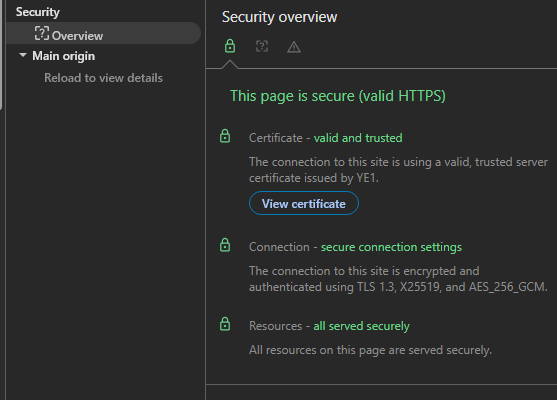
\includegraphics[width=0.51\linewidth,height=0.42\textheight,keepaspectratio]{figures/chrome-https.png}
\caption*{\textbf{ภาพที่ 4.1} Chrome ยืนยันว่าใบรับรองถูกต้องและเชื่อถือได้ และเชื่อมต่อด้วย TLS 1.3}
\end{figure}

\subsection*{4.1.5 SSH}

สร้างไฟล์ /etc/ssh/sshd\_config.d/00-hardening.conf ซึ่งถูกอ่านก่อนไฟล์อื่นในโฟลเดอร์เดียวกัน ค่าในไฟล์นี้จึงมีผลเสมอ

\begin{Verbatim}[breaklines,breakanywhere,fontsize=\small,frame=single,framesep=6pt]
PermitRootLogin no
PasswordAuthentication no
AuthenticationMethods publickey
\end{Verbatim}

ก่อนรีโหลด sshd สคริปต์ตรวจไวยากรณ์ด้วย sshd -t เพื่อไม่ให้ไฟล์ตั้งค่าผิดจนเข้าเครื่องไม่ได้

\begin{figure}[!htbp]
\centering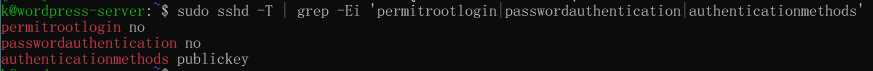
\includegraphics[width=0.79\linewidth,height=0.42\textheight,keepaspectratio]{figures/sshd-t.png}
\caption*{\textbf{ภาพที่ 4.2} ค่าที่ sshd ใช้งานจริง: ปิด root ปิดรหัสผ่าน และยืนยันตัวตนด้วยกุญแจเท่านั้น}
\end{figure}

\begin{figure}[!htbp]
\centering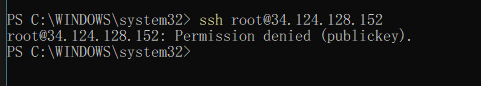
\includegraphics[width=0.50\linewidth,height=0.42\textheight,keepaspectratio]{figures/ssh-root-denied.png}
\caption*{\textbf{ภาพที่ 4.3} ทดสอบ ssh ด้วยบัญชี root จากเครื่องภายนอก ได้ Permission denied (publickey)}
\end{figure}

\subsection*{4.1.6 fail2ban, อัปเดตอัตโนมัติ และสำรองข้อมูล}

\begingroup\small\begin{longtable}[]{@{}>{\raggedright\arraybackslash}p{0.321\linewidth - 2\tabcolsep}>{\raggedright\arraybackslash}p{0.649\linewidth - 2\tabcolsep}@{}}
\toprule\noalign{}
รายการ & การตั้งค่า \\
\midrule\noalign{}
\endhead
\bottomrule\noalign{}
\endlastfoot
fail2ban (ค่าเริ่มต้น) & ผิด 5 ครั้งใน 10 นาที แบน 1 ชั่วโมง \\
jail sshd & อ่าน log จาก systemd journal \\
jail wordpress-login & นับการ login ผิดจาก access log ของ nginx ผิด 6 ครั้งแบน \\
jail nginx-limit-req & แบน IP ที่ถูก rate limit ซ้ำ \\
unattended-upgrades & ติดตั้งแพตช์ความปลอดภัยอัตโนมัติ \\
wp-backup.sh & สำรองฐานข้อมูลและไฟล์เว็บทุกวัน 03:30 น. เก็บ 7 วันที่ /var/backups/wordpress \\
\end{longtable}\endgroup

\begin{figure}[!htbp]
\centering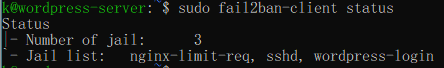
\includegraphics[width=0.50\linewidth,height=0.42\textheight,keepaspectratio]{figures/fail2ban-status.png}
\caption*{\textbf{ภาพที่ 4.4} fail2ban ทำงาน 3 jail: nginx-limit-req, sshd และ wordpress-login}
\end{figure}

\section*{4.2 ขั้นที่ 2: Geo-firewall รับเฉพาะ IP ไทย}\addcontentsline{toc}{section}{4.2 ขั้นที่ 2: Geo-firewall รับเฉพาะ IP ไทย}

\subsection*{4.2.1 การสร้างรายการ IP ไทย}

geo-firewall.sh ดาวน์โหลดไฟล์ delegated-apnic-latest จาก APNIC เลือกเฉพาะบรรทัดที่เป็น TH และ ipv4 แล้วแปลงจำนวน IP ของแต่ละช่วงเป็นรูป CIDR ด้วย Python ได้ 1,167 ช่วง หากดาวน์โหลดไม่ได้จะใช้ ipdeny.com เป็นแหล่งสำรอง และถ้าได้รายการน้อยผิดปกติสคริปต์จะหยุดทันที ไม่เปิด firewall ที่จะบล็อกทุกคน

รายการถูกโหลดเข้า ipset ชื่อ geo\_TH แบบ hash:net โดยสร้างชุดชั่วคราวก่อนแล้วสลับ (ipset swap) ทำให้อัปเดตได้โดยไม่มีช่วงเวลาที่ชุดว่าง

\subsection*{4.2.2 กฎ iptables}

\begin{Verbatim}[breaklines,breakanywhere,fontsize=\small,frame=single,framesep=6pt]
iptables -N GEO_IN
iptables -A GEO_IN -i lo -j RETURN
iptables -A GEO_IN -m conntrack --ctstate ESTABLISHED,RELATED -j RETURN
iptables -A GEO_IN -s 169.254.169.254 -j RETURN        # metadata ของ cloud
iptables -A GEO_IN -s 10.0.0.0/8 -j RETURN             # เครือข่ายภายในของ cloud
iptables -A GEO_IN -m set --match-set geo_TH src -j RETURN
iptables -A GEO_IN -m limit --limit 5/min -j LOG --log-prefix "GEO-BLOCK: "
iptables -A GEO_IN -j DROP
iptables -I INPUT 1 -j GEO_IN
\end{Verbatim}

กฎทำงานตามลำดับ แพ็กเก็ตของการเชื่อมต่อที่เครื่องเริ่มเอง (เช่น การอัปเดตแพ็กเกจ หรือการเรียก API) ผ่านด้วยกฎ ESTABLISHED,RELATED ส่วนการเชื่อมต่อใหม่จากภายนอกผ่านได้เฉพาะ IP ที่อยู่ใน geo\_TH ที่เหลือจะถูกบันทึก log (จำกัด 5 บรรทัดต่อนาที กัน log ล้น) แล้ว DROP

\subsection*{4.2.3 การป้องกันการล็อกตัวเองออก}

\begin{itemize}
\tightlist
\item
  ก่อนเปิด สคริปต์ตรวจว่า IP ที่กำลัง SSH อยู่อยู่ในชุด IP ไทย ถ้าไม่อยู่จะไม่ยอมเปิด
\item
  คำสั่ง apply ตั้งตัวจับเวลา 3 นาที ถ้าผู้ดูแลไม่พิมพ์ confirm ภายในเวลานั้น ระบบจะปิด firewall เอง กรณีตั้งค่าผิดจนเข้าเครื่องไม่ได้
\item
  บริการ systemd เปิด firewall ใหม่ทุกครั้งที่รีบูต และ cron อัปเดตรายการ IP ทุกสัปดาห์
\item
  คำสั่งที่ใช้ได้: apply, confirm, status, update, off
\end{itemize}

\begin{figure}[!htbp]
\centering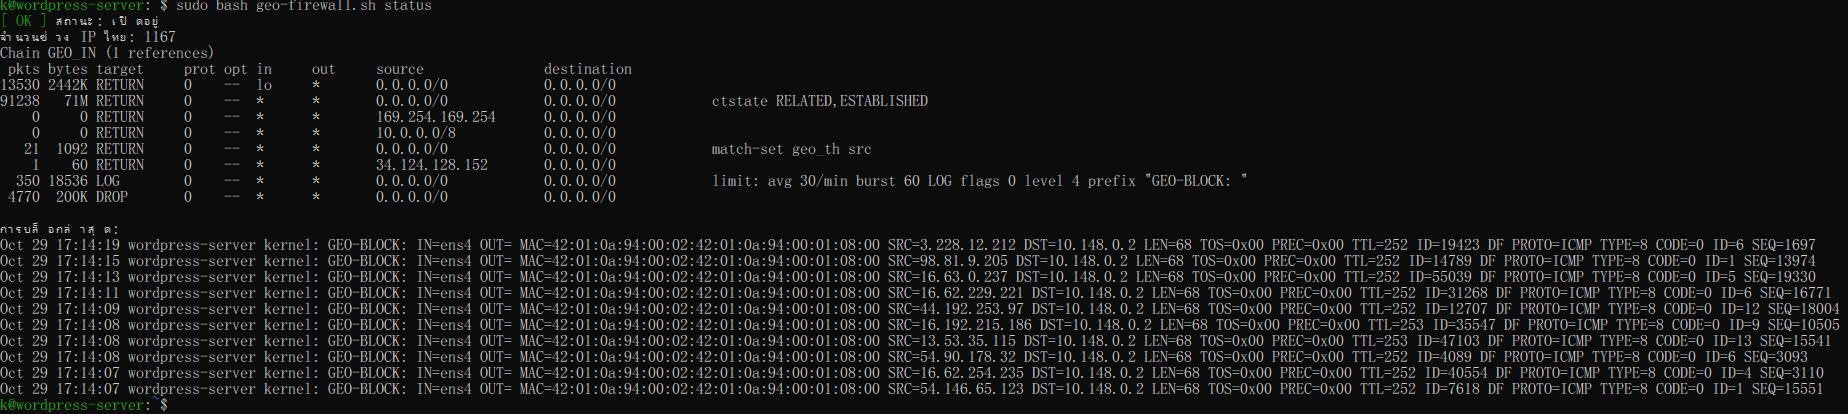
\includegraphics[width=1.00\linewidth,height=0.42\textheight,keepaspectratio]{figures/geo-firewall-status.png}
\caption*{\textbf{ภาพที่ 4.5} สถานะ geo-firewall: ช่วง IP ไทย 1,167 ช่วง กฎ chain GEO\_IN (รวมกฎอนุญาต IP ของเซิร์ฟเวอร์เอง) และ log GEO-BLOCK ล่าสุด}
\end{figure}

\section*{4.3 ขั้นที่ 3: เว็บไซต์สาขาวิทยาการคอมพิวเตอร์}\addcontentsline{toc}{section}{4.3 ขั้นที่ 3: เว็บไซต์สาขาวิทยาการคอมพิวเตอร์}

\subsection*{4.3.1 ธีม}

คณะผู้จัดทำเขียนธีม BUU Computer Science ขึ้นเองตามแบบที่ทีมออกแบบไว้ใน Figma ใช้โทนสีฟ้ากับกรมท่า (\#0a2e57, \#0b6fd0) ฟอนต์ Anuphan และ IBM Plex Sans Thai ออกแบบให้อ่านง่ายบนโทรศัพท์ เนื่องจากกลุ่มเป้าหมายส่วนใหญ่เป็นนักเรียนมัธยมที่ใช้มือถือเป็นหลัก

หน้าหลักของเว็บไซต์

\begingroup\small\begin{longtable}[]{@{}>{\raggedright\arraybackslash}p{0.310\linewidth - 2\tabcolsep}>{\raggedright\arraybackslash}p{0.660\linewidth - 2\tabcolsep}@{}}
\toprule\noalign{}
หน้า & เนื้อหา \\
\midrule\noalign{}
\endhead
\bottomrule\noalign{}
\endlastfoot
หน้าแรก & แนะนำสาขา จุดเด่น หลักสูตร อาชีพหลังจบ ข่าวล่าสุด \\
เกี่ยวกับสาขา & แสดงเนื้อหาที่แก้ได้จากตัวแก้ไขบทความ \\
ข่าวสารและกิจกรรม & ข่าวที่นำเข้าจากเว็บไซต์คณะ \\
หลักสูตร & หลักสูตรและรายละเอียดของสาขา \\
\end{longtable}\endgroup

\begin{figure}[!htbp]
\centering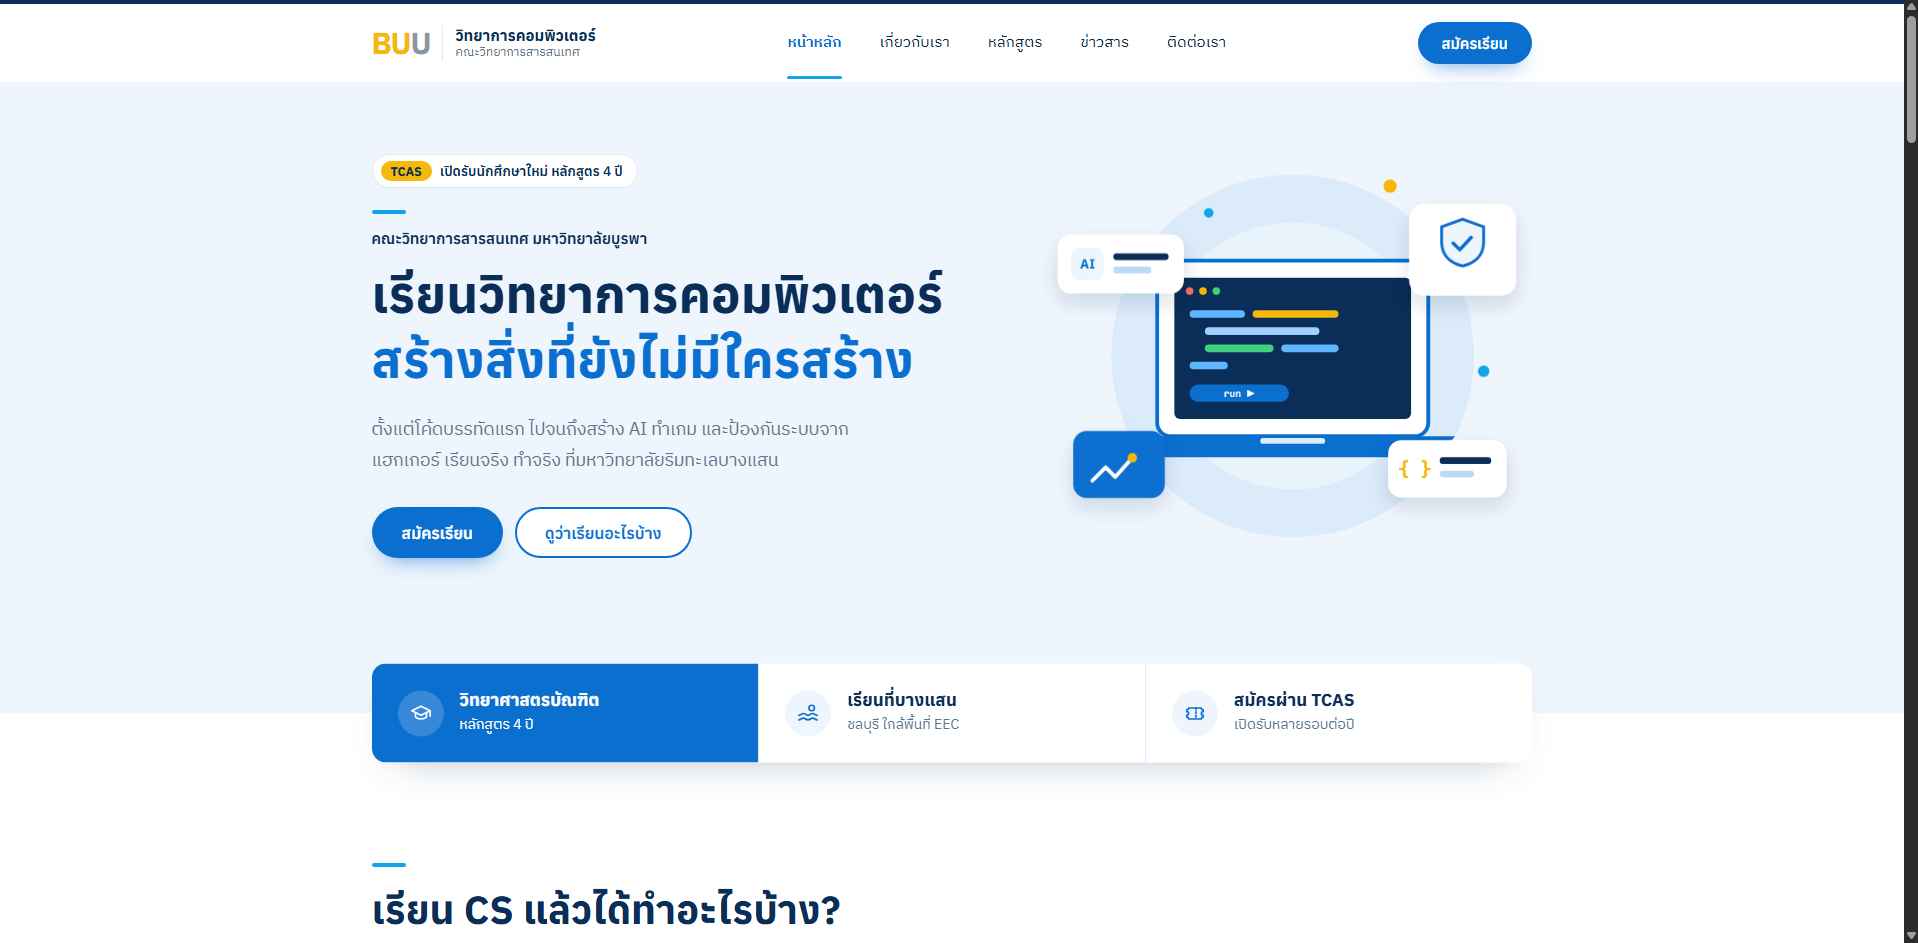
\includegraphics[width=1.00\linewidth,height=0.42\textheight,keepaspectratio]{figures/home-desktop.png}
\caption*{\textbf{ภาพที่ 4.6} หน้าแรกของเว็บไซต์บนคอมพิวเตอร์}
\end{figure}

\begin{figure}[!htbp]
\centering
\includegraphics[width=0.84\linewidth,height=0.42\textheight,keepaspectratio]{figures/home-mobile.png}
\caption*{\textbf{ภาพที่ 4.7} หน้าแรกบนมือถือ เมนูยุบเป็นปุ่ม และข้อความปรับขนาดให้อ่านง่าย}
\end{figure}

\subsection*{4.3.2 เนื้อหาที่แก้ไขได้จากหลังบ้าน}

ข้อความทุกส่วนของธีมถูกกำหนดเป็นค่าตั้ง (setting) ใน WordPress Customizer ภายใต้แผง ``เนื้อหาเว็บไซต์'' ประมาณ 10 หมวด รวม 101 ค่า สมาชิกทีมแก้ข้อความและเห็นผลทันทีโดยไม่ต้องแก้โค้ด ถ้าลบหัวข้อของส่วนใดออก ส่วนนั้นจะซ่อนอัตโนมัติ ข้อความทุกจุดผ่านฟังก์ชัน escape ก่อนแสดงผล เพื่อป้องกัน XSS

\begin{figure}[!htbp]
\centering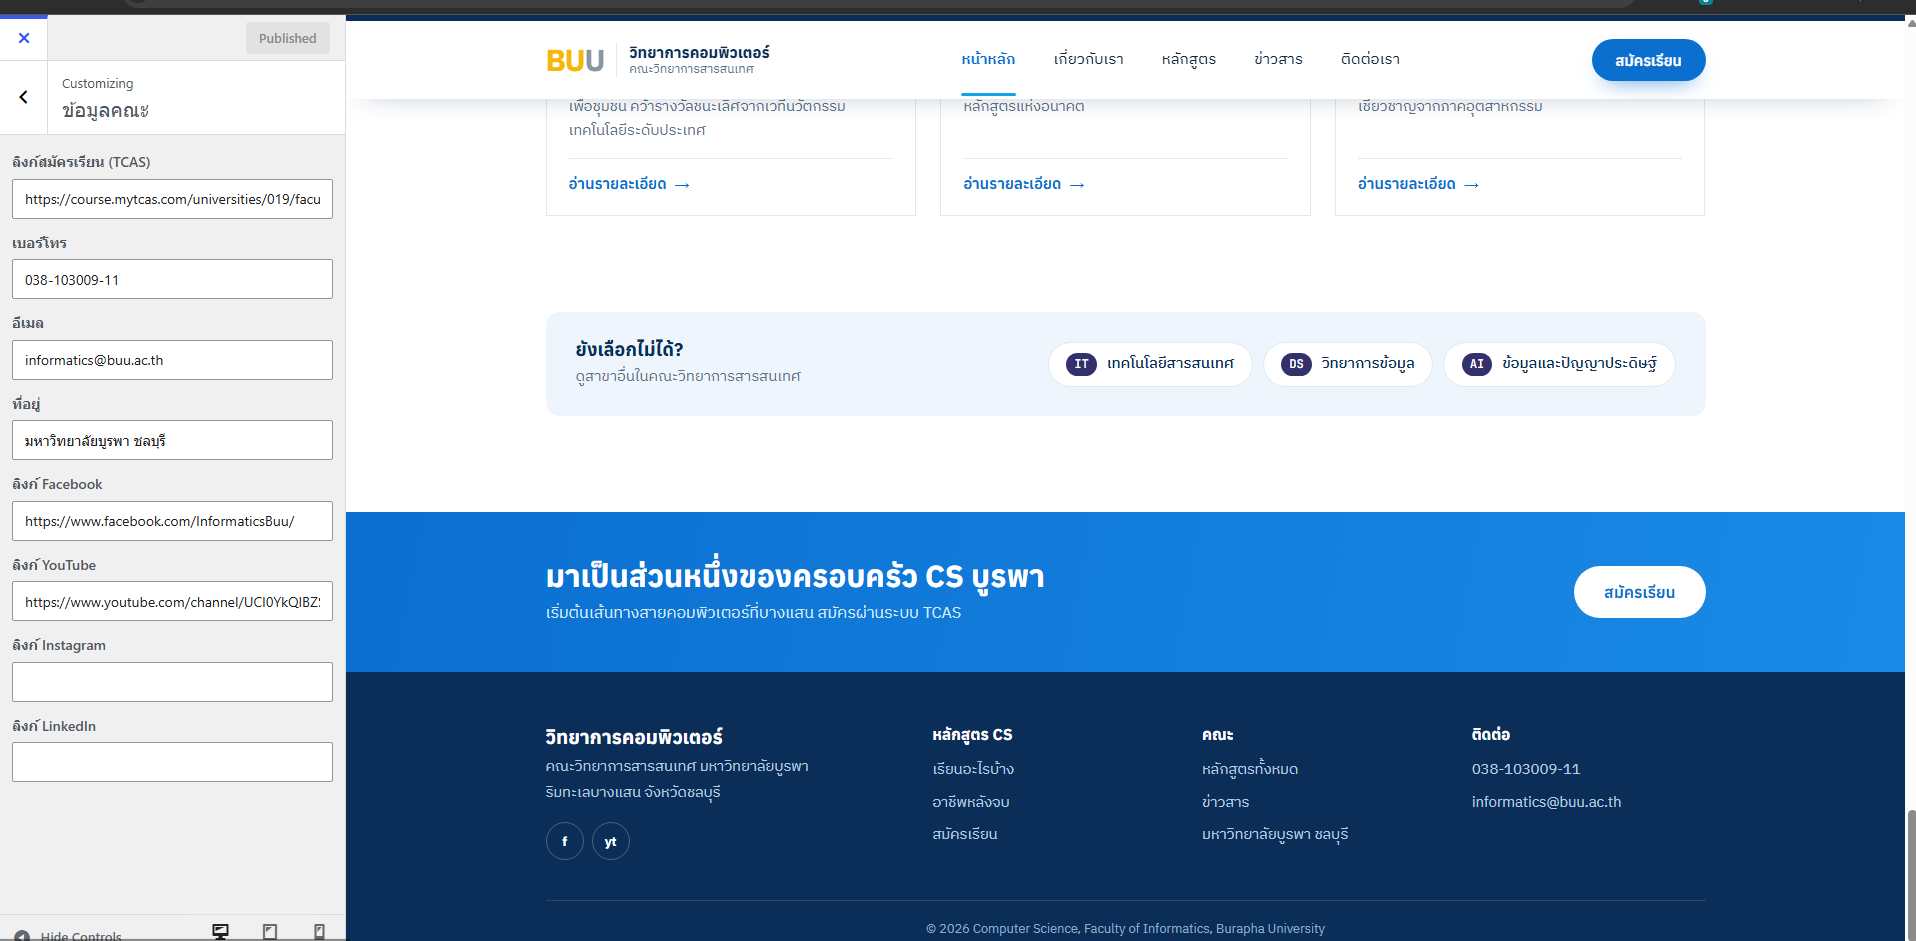
\includegraphics[width=1.00\linewidth,height=0.42\textheight,keepaspectratio]{figures/customizer.png}
\caption*{\textbf{ภาพที่ 4.8} แก้ข้อความของเว็บไซต์ได้จาก Customizer โดยไม่ต้องแก้โค้ด}
\end{figure}

\subsection*{4.3.3 การนำเข้าข่าวจากเว็บไซต์คณะ}

เว็บไซต์คณะใช้ WordPress และเปิด REST API (?rest\_route=/wp/v2/posts) ไว้ คณะผู้จัดทำจึงดึงข้อมูลผ่าน API แทนการสแครปหน้าเว็บ ได้ข้อมูลที่มีโครงสร้างและไม่พังเมื่อหน้าตาเว็บคณะเปลี่ยน หาก API ใช้ไม่ได้จะใช้ RSS feed แทน

\begin{enumerate}
\def\labelenumi{\arabic{enumi}.}
\tightlist
\item
  WP-Cron เรียก buu\_import\_news() ทุกชั่วโมง
\item
  ดึงรายการข่าวผ่าน REST API นำเข้าใหม่ได้ครั้งละไม่เกิน 25 ข่าว รวมสูงสุด 100 ข่าว
\item
  ตรวจข่าวซ้ำจาก meta \_buu\_src ที่เก็บลิงก์ต้นทาง
\item
  กรองเนื้อหาด้วย wp\_kses\_post (ตัดสคริปต์และแท็กอันตราย) และต่อท้ายด้วยบรรทัดเครดิตแหล่งที่มา
\item
  ดาวน์โหลดรูปปกเฉพาะลิงก์ https เก็บเป็นไฟล์ในเว็บของเราเอง
\item
  บันทึกเป็นโพสต์ในตาราง wp\_posts และแสดงในหน้าข่าวสาร
\end{enumerate}

ผู้ดูแลสั่งนำเข้าทันทีได้จากเมนู Tools ในหลังบ้าน และตรวจข้อมูลในฐานข้อมูลได้ด้วย DBeaver ผ่าน SSH tunnel เช่น

\begin{Verbatim}[breaklines,breakanywhere,fontsize=\small,frame=single,framesep=6pt]
SELECT p.ID, p.post_title, p.post_date, m.meta_value AS source_url
FROM wp_posts p
JOIN wp_postmeta m ON m.post_id = p.ID AND m.meta_key = '_buu_src'
WHERE p.post_type = 'post'
ORDER BY p.post_date DESC;
\end{Verbatim}

\begin{figure}[!htbp]
\centering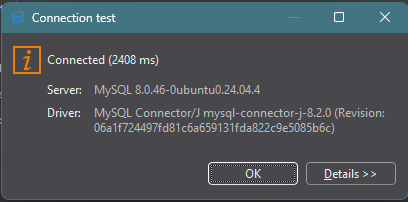
\includegraphics[width=0.50\linewidth,height=0.42\textheight,keepaspectratio]{figures/dbeaver.png}
\caption*{\textbf{ภาพที่ 4.9} DBeaver เชื่อมต่อ MySQL 8.0.46 ผ่าน SSH tunnel สำเร็จ}
\end{figure}

\begin{figure}[!htbp]
\centering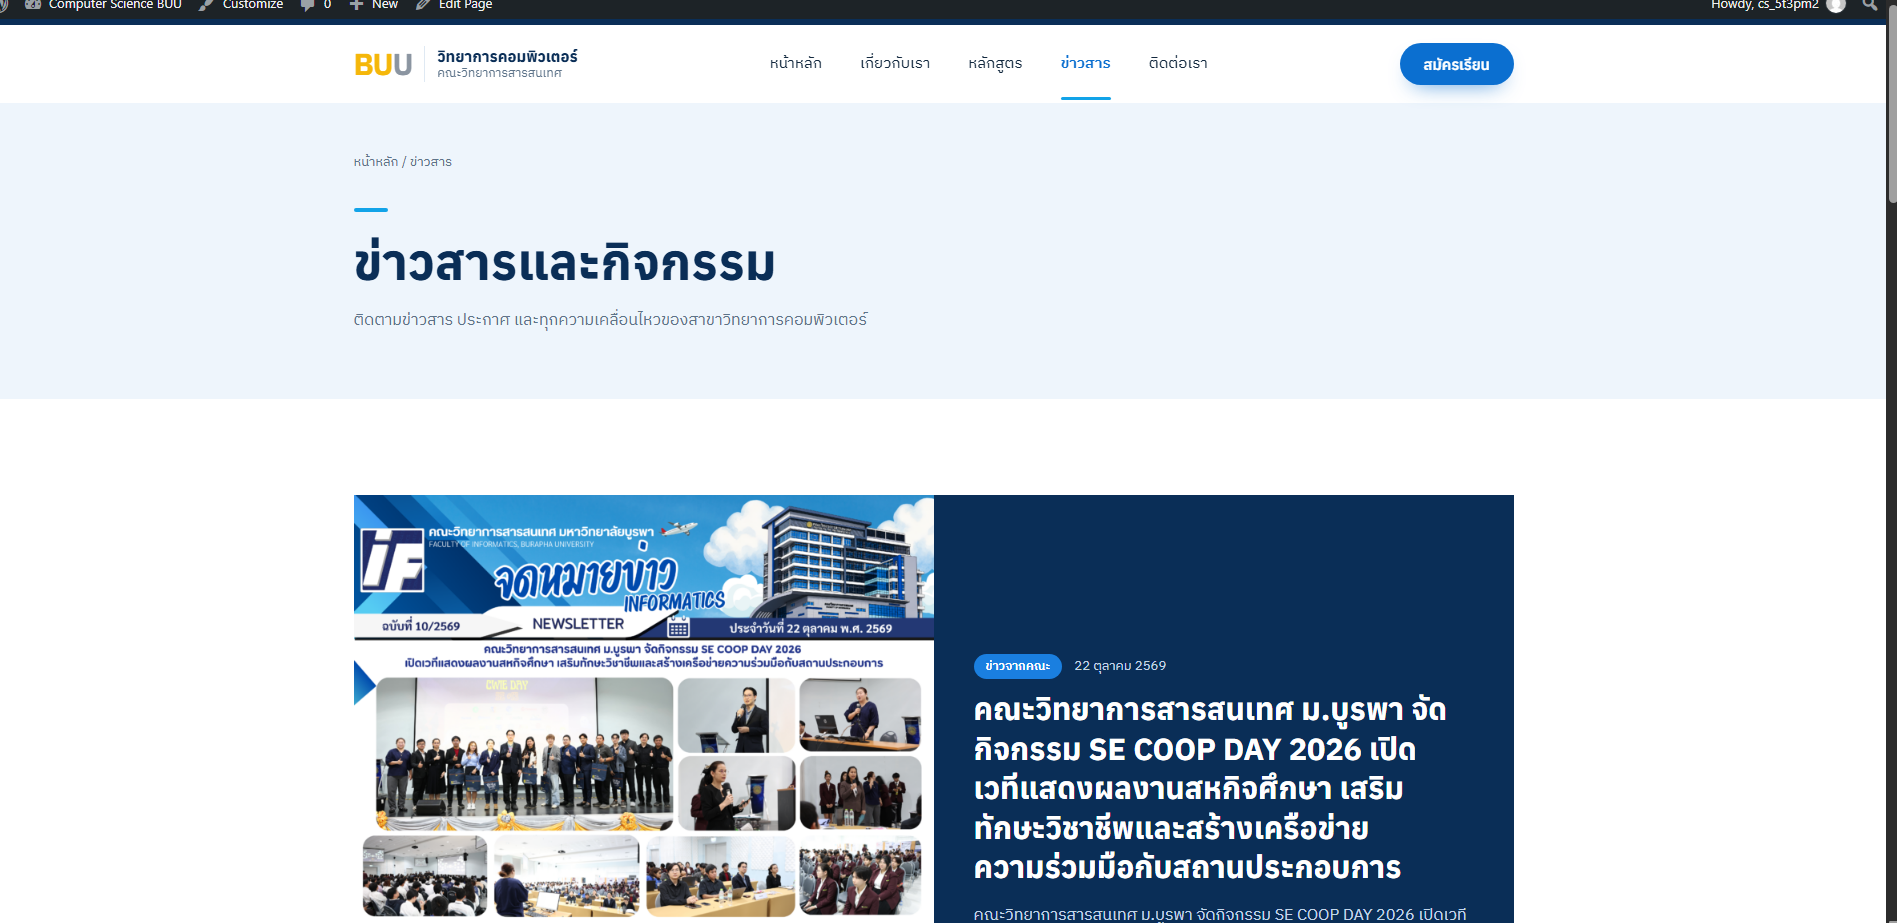
\includegraphics[width=1.00\linewidth,height=0.42\textheight,keepaspectratio]{figures/news-page.png}
\caption*{\textbf{ภาพที่ 4.10} หน้าข่าวสารและกิจกรรมที่แสดงข่าวที่นำเข้าจากเว็บไซต์คณะ}
\end{figure}

\subsection*{4.3.4 บัญชีผู้ใช้และ 2FA}

ผู้ดูแลเปิด 2FA ด้วยปลั๊กอิน Two-Factor สมาชิกคนอื่นได้บัญชีสิทธิ์ Editor ที่แก้เนื้อหาได้ แต่ติดตั้งปลั๊กอินหรือเปลี่ยนการตั้งค่าไม่ได้ ธีมและปลั๊กอินที่ไม่ได้ใช้ถูกลบออก เหลือเฉพาะธีมของคณะผู้จัดทำและปลั๊กอิน Two-Factor

\section*{4.4 การตรวจความปลอดภัยช่วงช่องโหว่ PHP (ต.ค. 2569)}\addcontentsline{toc}{section}{4.4 การตรวจความปลอดภัยช่วงช่องโหว่ PHP (ต.ค. 2569)}

ปลายเดือนตุลาคม 2569 มีการประกาศช่องโหว่ร้ายแรงใน PHP คือ CVE-2026-109618 และ CVE-2026-109619 ซึ่งทำให้ผู้โจมตีรันโค้ดบนเซิร์ฟเวอร์ได้โดยไม่ต้องล็อกอิน และถูกนำไปใช้โจมตีจริงแล้ว รวมถึง CVE-2026-115560 ที่ยังไม่มีแพตช์ คณะผู้จัดทำจึงเขียนสคริปต์ security-check.sh เพื่อตรวจและแก้ไข

\begingroup\small\begin{longtable}[]{@{}>{\raggedright\arraybackslash}p{0.275\linewidth - 2\tabcolsep}>{\raggedright\arraybackslash}p{0.695\linewidth - 2\tabcolsep}@{}}
\toprule\noalign{}
รายการ & วิธีตรวจ/แก้ \\
\midrule\noalign{}
\endhead
\bottomrule\noalign{}
\endlastfoot
แพตช์ PHP & ตรวจว่า php8.3-fpm เป็นเวอร์ชัน 8.3.6-0ubuntu0.24.04.13 ขึ้นไป (USN-8948-1) เพราะ php -v แสดงแค่ 8.3.6 จึงใช้ยืนยันไม่ได้ แล้วรีสตาร์ต PHP-FPM ให้ worker ใช้โค้ดใหม่ \\
CVE-2026-115560 & ปิด session.upload\_progress.enabled ในการตั้งค่าของ PHP-FPM (WordPress ไม่ได้ใช้) \\
จำกัดความเสียหาย & ปิดฟังก์ชันรันคำสั่งระบบ (exec, system, shell\_exec, proc\_open, popen) ใน PHP-FPM \\
ตรวจการบุกรุก & หาไฟล์ PHP ในโฟลเดอร์ uploads, ไฟล์ PHP ที่ถูกแก้ใน 7 วัน, ตรวจไฟล์ WordPress core และปลั๊กอินกับต้นฉบับ (wp core verify-checksums) \\
มุมมองคนนอก & ทดสอบว่า xmlrpc.php, .env, ?author=1 และ REST รายชื่อผู้ใช้ ถูกปฏิเสธ \\
ระบบ & พอร์ตที่เปิด, MySQL รับเฉพาะ 127.0.0.1, SSH, fail2ban, geo-firewall, อัปเดตที่ค้าง \\
\end{longtable}\endgroup

นอกจากนี้ธีมเวอร์ชัน 3.7.0 เพิ่มไฟล์ inc/hardening.php ปิดการไล่หาชื่อผู้ใช้สำหรับคนที่ไม่ได้ล็อกอิน (?author=N ได้ 403, REST /wp/v2/users ถูกซ่อน, sitemap และ oEmbed ไม่แสดงผู้เขียน) ซ่อนเวอร์ชัน WordPress และใช้ข้อความล็อกอินผิดแบบไม่บอกว่าชื่อผู้ใช้มีอยู่จริงหรือไม่

ผลการรัน security-check.sh บนเซิร์ฟเวอร์จริง (29 ตุลาคม 2569)

\begin{figure}[!htbp]
\centering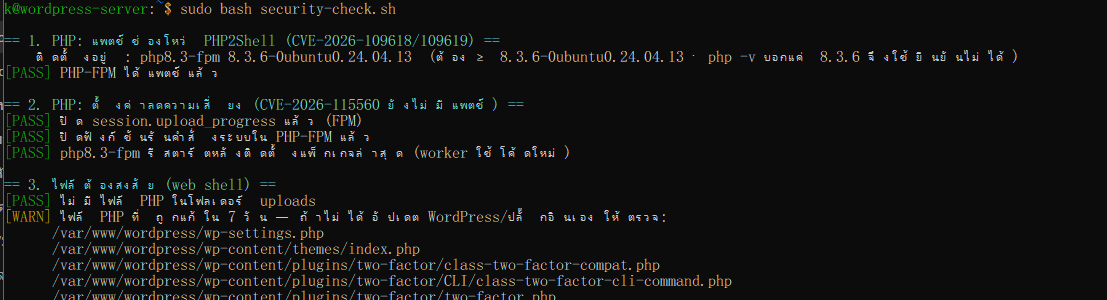
\includegraphics[width=1.00\linewidth,height=0.42\textheight,keepaspectratio]{figures/security-check-php.png}
\caption*{\textbf{ภาพที่ 4.11} PHP-FPM ได้แพตช์แล้ว (8.3.6-0ubuntu0.24.04.13) และตั้งค่าลดความเสี่ยงครบ}
\end{figure}

\begin{figure}[!htbp]
\centering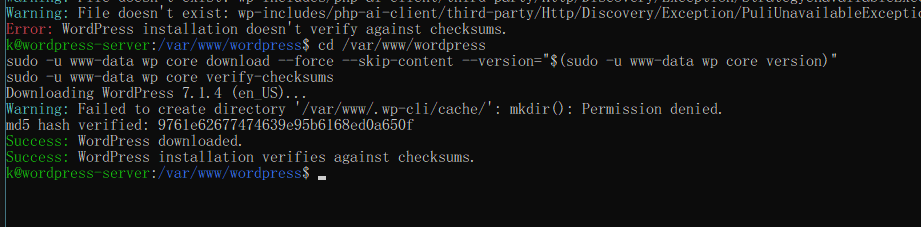
\includegraphics[width=0.84\linewidth,height=0.42\textheight,keepaspectratio]{figures/wp-checksums.png}
\caption*{\textbf{ภาพที่ 4.12} หลังดาวน์โหลด core ทับใหม่ ไฟล์ WordPress ทุกไฟล์ตรงกับต้นฉบับจาก wordpress.org}
\end{figure}

\begin{figure}[!htbp]
\centering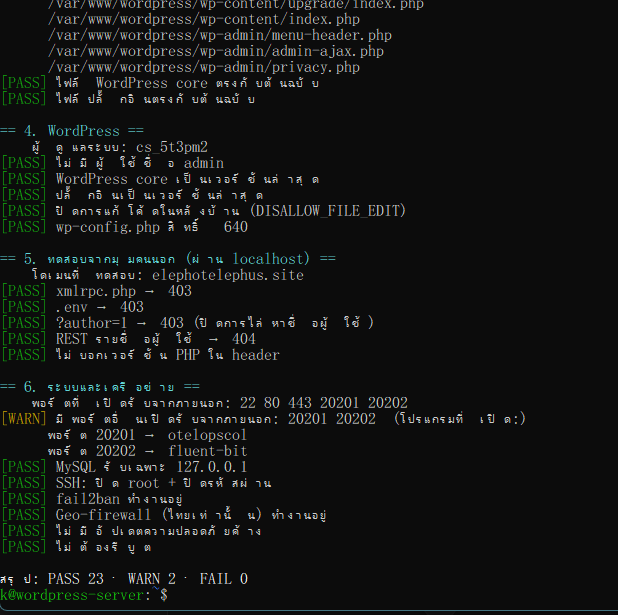
\includegraphics[width=0.56\linewidth,height=0.42\textheight,keepaspectratio]{figures/security-check-summary.png}
\caption*{\textbf{ภาพที่ 4.13} ผลสรุป PASS 23 · WARN 2 · FAIL 0 โดย WARN ทั้งสองข้อตรวจแล้วอธิบายได้ คือไฟล์ที่เปลี่ยนจากการอัปเดต (ตรงกับต้นฉบับ) และพอร์ต 20201/20202 ของ Google Cloud Ops Agent ซึ่งคนภายนอกเข้าไม่ถึง}
\end{figure}